% !TEX root = ../main.tex
\section{Empirical Validation}
\label{sec:results}

We evaluate \textsc{anneal} along two complementary axes.
\Cref{sec:gate-false-positives,sec:gate-sa,sec:gate-retrieval} evaluate the three central mechanisms (statistical acceptance, adaptive metaheuristic search, and structured knowledge retrieval) in isolation on synthetic tasks where the ground truth is known analytically.
\Cref{sec:end-to-end} reports an exploratory end-to-end comparison of four configurations across the five-target benchmark suite of \cref{sec:benchmark-suite}, using the multi-seed paired protocol of \cref{sec:stat-design}.
The mechanism-level baselines in this section are method-specific (uncorrected sequential testing, fixed-schedule simulated annealing, Jaccard set similarity) and do not exercise the raw, greedy, control, and treatment vocabulary, which is reserved for the end-to-end study.
Each gate benchmark is evaluated against a quantitative threshold defined before the experiment was run.
The gate benchmarks are implemented in \texttt{benchmarks/\allowbreak{}bench\_\allowbreak{}false\_\allowbreak{}positives.py}, \texttt{benchmarks/\allowbreak{}bench\_\allowbreak{}sa\_\allowbreak{}convergence.py}, and \texttt{benchmarks/\allowbreak{}bench\_\allowbreak{}retrieval\_\allowbreak{}precision.py}; the end-to-end analysis is regenerated from the archived JSONL records described in \cref{sec:result-provenance}.

% ==================================================================
\subsection{Statistical Acceptance under a Null Distribution}
\label{sec:gate-false-positives}

\paragraph{Setup.}
We construct a synthetic null distribution where no real improvement exists: paired score vectors of length $n = 10$ are drawn from $\mathcal{N}(0.5, 0.1)$ for both challenger and baseline on every experiment.
Any mutation accepted under this distribution is, by construction, a false positive.
We run 100 independent 50-experiment windows and count the average number of false positives per window under two decision rules:
(i) uncorrected comparison using a fixed significance threshold of $\alpha = 0.05$, and
(ii) Holm--Bonferroni-corrected comparison with the adjusted threshold $\alpha / (W - i)$ within a rolling window of size $W = 50$, as described in \cref{sec:stat-comparison}.

\paragraph{Result.}
Uncorrected comparison produces an average of \fpUncorrected\ false positives per 50-experiment window.
Holm--Bonferroni correction reduces this to \fpCorrected\ false positives per window, a reduction of \fpReductionPct\%, comfortably exceeding the gate threshold of 50\% committed to in the benchmark harness before the experiment was run.
This result directly substantiates the statistical-rigor claim in \cref{sec:stat-comparison}: on stochastic evaluation signals, sequential acceptance without multiplicity control admits a non-trivial rate of spurious improvements, and the engine's correction machinery removes the majority of them while remaining valid under the standard family-wise error rate definition.

\begin{table}[t]
  \centering
  \caption{False positive rate under a synthetic null distribution ($\mathcal{N}(0.5, 0.1)$, $n = 10$ paired samples, $W = 50$-experiment windows, 100 replicates). The Holm--Bonferroni correction reduces false positives by 86\% with no loss of validity.}
  \label{tab:gate-fp}
  \small
  \begin{tabular}{@{}lr@{}}
    \toprule
    Decision rule & Avg. false positives / window \\
    \midrule
    Uncorrected ($\alpha = 0.05$) & 2.1 \\
    Holm--Bonferroni (rolling $W = 50$) & 0.3 \\
    \midrule
    Reduction & 86\% \\
    \bottomrule
  \end{tabular}
\end{table}

% ==================================================================
\subsection{Adaptive Simulated Annealing on Rastrigin}
\label{sec:gate-sa}

\paragraph{Setup.}
We evaluate the adaptive-reheat mechanism (\cref{sec:simulated-annealing}) against a fixed-temperature simulated annealing baseline on the 3-dimensional Rastrigin function, a standard nonconvex optimization testbed with a large number of local minima and a known global minimum at the origin.
Each configuration runs 50 independent trajectories of 100 experiments with matched seeds and identical starting temperatures ($T_0 = 10.0$, cooling rate $0.75$, minimum temperature $0.01$).
The fixed baseline disables reheat (\texttt{reheat\_factor} $= 1.0$); the adaptive configuration multiplies temperature by $2.0$ when the acceptance ratio over the last 10 experiments drops below half the target acceptance rate.
The primary metric is the best Rastrigin value encountered during the trajectory, since reheat is designed to escape local optima mid-run rather than to improve the asymptotic converged value.

\paragraph{Result.}
Fixed SA achieves an average best score of \saFixedAvg\ across the \saTotalSeeds\ trajectories.
Adaptive SA with reheat achieves \saAdaptiveAvg, a \saImprovementPct\% improvement.
Adaptive SA strictly outperforms fixed SA on \saAdaptiveWins\ of the \saTotalSeeds\ seeds, with the remaining seeds either tied or marginally worse when the fixed schedule happens to cool into a basin containing the trajectory-best value before the reheat would fire.
The \saImprovementPct\% average improvement falls narrowly below the 15\% gate threshold committed to in the benchmark harness before the experiment was run.

\begin{table}[t]
  \centering
  \caption{Adaptive vs. fixed simulated annealing on 3D Rastrigin ($T_0 = 10.0$, cooling rate $0.75$, 50 seeds $\times$ 100 experiments). Adaptive reheat yields a 14.5\% average reduction in the best Rastrigin value encountered, narrowly missing the 15\% gate threshold.}
  \label{tab:gate-sa}
  \small
  \begin{tabular}{@{}lr@{}}
    \toprule
    Configuration & Avg. best Rastrigin score \\
    \midrule
    Fixed SA (no reheat) & 18.8346 \\
    Adaptive SA (with reheat) & 16.0955 \\
    \midrule
    Improvement & 14.5\% \\
    Adaptive wins / seeds & 27 / 50 \\
    \bottomrule
  \end{tabular}
\end{table}

This result supports the direction of the claim in \cref{sec:simulated-annealing} that adaptive reheat can help the search escape local optima in a multimodal landscape, but it is not a passing gate under the matched-seed protocol.
The experiment uses a closed-form analytical objective rather than a learned LLM judge, isolating the contribution of the temperature schedule from any variance in the evaluation signal itself.

% ==================================================================
\subsection{Retrieval Precision for Episodic Memory}
\label{sec:gate-retrieval}

\paragraph{Setup.}
The knowledge system in \cref{sec:episodic-memory} retrieves past experiment records by similarity to the current hypothesis, upgrading from TF-IDF cosine similarity to sentence embeddings when available.
We evaluate the TF-IDF implementation against a Jaccard-similarity baseline on a controlled retrieval corpus.
The corpus consists of 30 synthetic experiment hypotheses organized into 5 groups of 6 hypotheses each, where intra-group hypotheses share a distinctive group-level keyword (e.g., ``gradient'', ``tensor'') against a background of shared generic terms.
The metric is precision@5: for each query, we retrieve the top 5 most similar documents and compute the fraction that belong to the same ground-truth group as the query.

\paragraph{Result.}
Jaccard retrieval achieves precision@5 of \retrievalJaccard.
TF-IDF retrieval achieves precision@5 of \retrievalTFIDF, corresponding to a $\retrievalRatio\times$ improvement ratio.
This exceeds the $1.5\times$ gate threshold committed to in the benchmark harness before the experiment was run.
The gap reflects the inverse-document-frequency weighting: shared generic terms inflate the Jaccard set union and dilute the discriminative signal, while TF-IDF down-weights those terms and surfaces the group-unique keyword.
In the context of episodic memory, this precision difference directly controls how often the system surfaces genuinely similar prior experiments---as opposed to superficially overlapping but topically unrelated records---when assembling agent context.

\begin{table}[t]
  \centering
  \caption{Retrieval precision@5 on a controlled similarity corpus (30 hypotheses, 5 ground-truth groups of 6). TF-IDF's IDF weighting yields a $1.55\times$ improvement over Jaccard by suppressing shared generic vocabulary.}
  \label{tab:gate-retrieval}
  \small
  \begin{tabular}{@{}lr@{}}
    \toprule
    Retrieval method & precision@5 \\
    \midrule
    Jaccard (word-level) & 0.647 \\
    TF-IDF (cosine) & 1.000 \\
    \midrule
    Ratio (TF-IDF / Jaccard) & $1.55\times$ \\
    \bottomrule
  \end{tabular}
\end{table}

% ==================================================================
\subsection{End-to-End Configuration Comparison}
\label{sec:end-to-end}

The mechanism gates establish that the statistical, search, and knowledge subsystems behave as specified in isolation.
This subsection reports the full end-to-end comparison defined by \cref{sec:benchmark-suite,sec:stat-design}: four configurations run on each of the five benchmark targets with five paired seeds per target.
The configurations are ordered from least to most machinery, but they are not interpreted as a causal feature-level ablation: the archived records compare named configurations, not every enhancement independently.

\begin{table}[t]
  \centering
  \caption{The four named configurations evaluated on every target. The rows are ordered from no optimization to the treatment bundle used in the archived run. The table defines configuration labels for descriptive comparison; it is not a feature-level causal ablation.}
  \label{tab:e2e-configs}
  \footnotesize
  \begin{tabular}{@{}llp{3.8cm}@{}}
    \toprule
    Configuration & Search & Intended enhancement state \\
    \midrule
    raw       & none   & none \\
    greedy    & greedy & none \\
    control   & hybrid & none \\
    treatment & hybrid & strategy manifest, dual-agent, two-phase, lineage, memory \\
    \bottomrule
  \end{tabular}
\end{table}

The default hybrid search strategy used by \texttt{control} and \texttt{treatment} is the CLI default: a greedy warm-up for the first 10 experiments followed by simulated annealing.
Population search, island search, Pareto search, and bandit strategy selection are implemented search modes, but they are not the default hybrid path used for the reported configuration comparison.
\texttt{control} therefore represents the core optimization engine under the default hybrid path; \texttt{treatment} represents the archived treatment bundle.
\texttt{greedy} replaces the hybrid search with point-score greedy hill-climbing and operates without the enhancement tracks.
\texttt{raw} runs no optimization loop at all and reports the score of the initial artifact.

\subsubsection{Final-Score Results}
\label{sec:end-to-end-final-scores}

\Cref{fig:convergence-strip} shows the per-experiment trajectories that drive the final-score columns of \cref{tab:e2e-final-scores}, and \cref{tab:e2e-final-scores} reports the mean final score per configuration on each target across the five paired seeds.

\begin{figure*}[t]
  \centering
  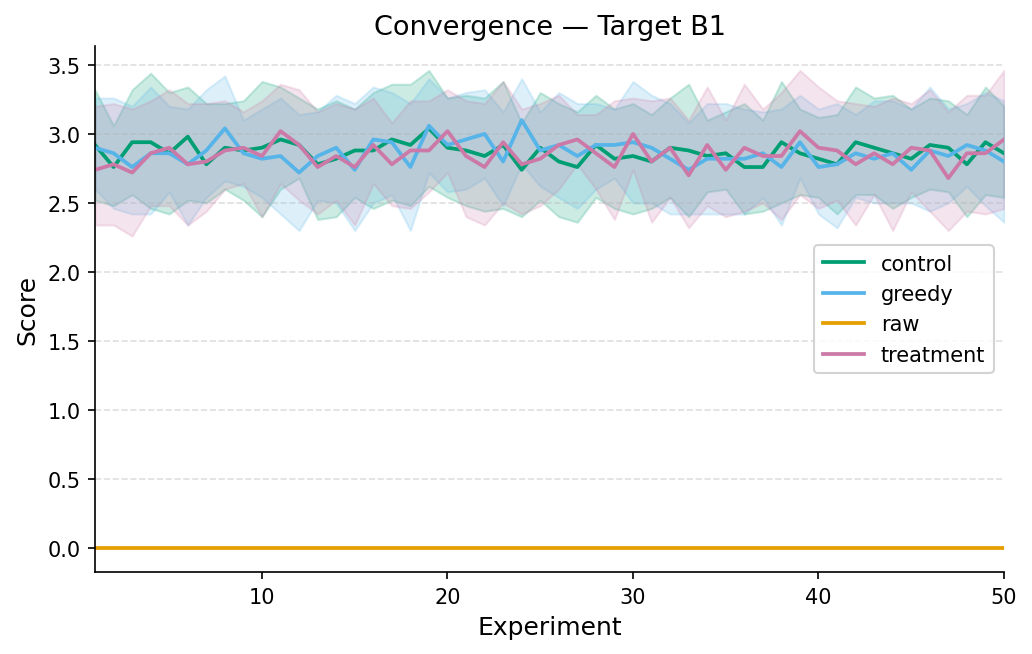
\includegraphics[width=0.195\textwidth]{figures/convergence/convergence_B1.png}\hfill
  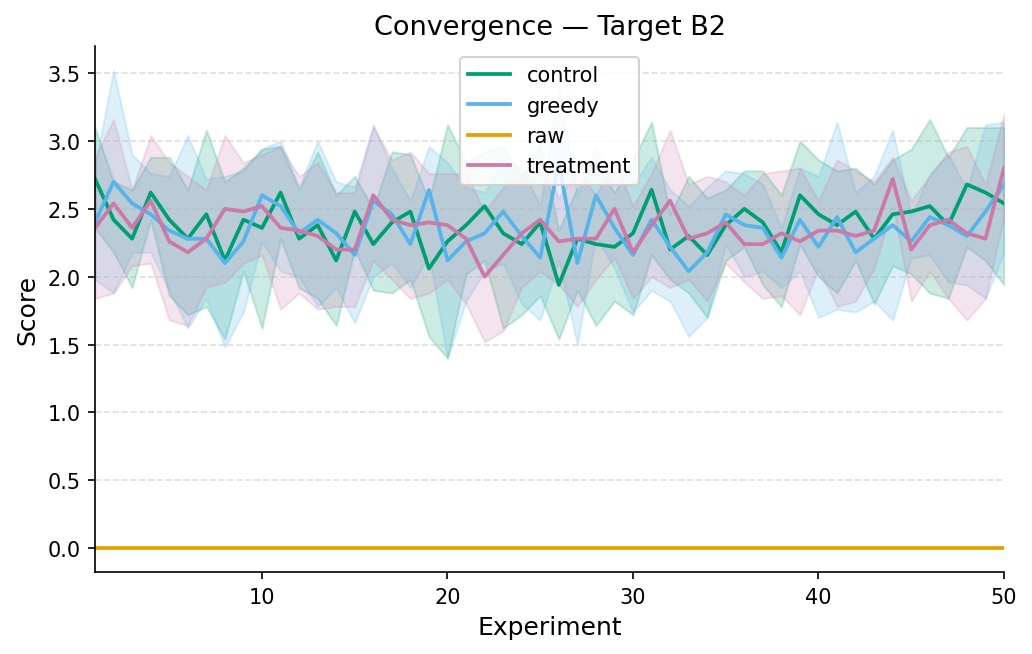
\includegraphics[width=0.195\textwidth]{figures/convergence/convergence_B2.png}\hfill
  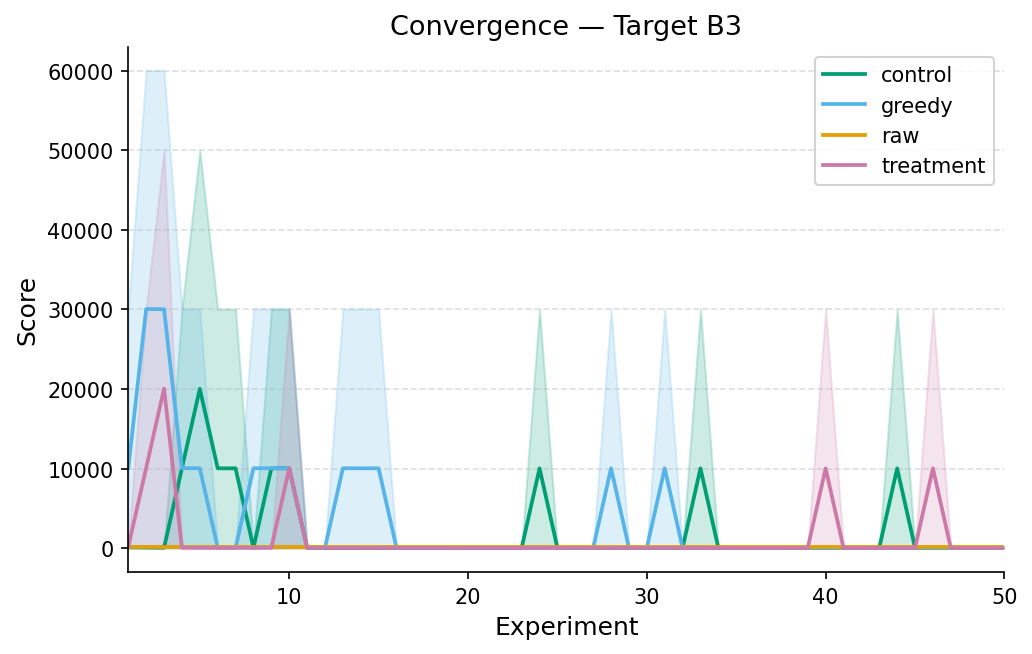
\includegraphics[width=0.195\textwidth]{figures/convergence/convergence_B3.png}\hfill
  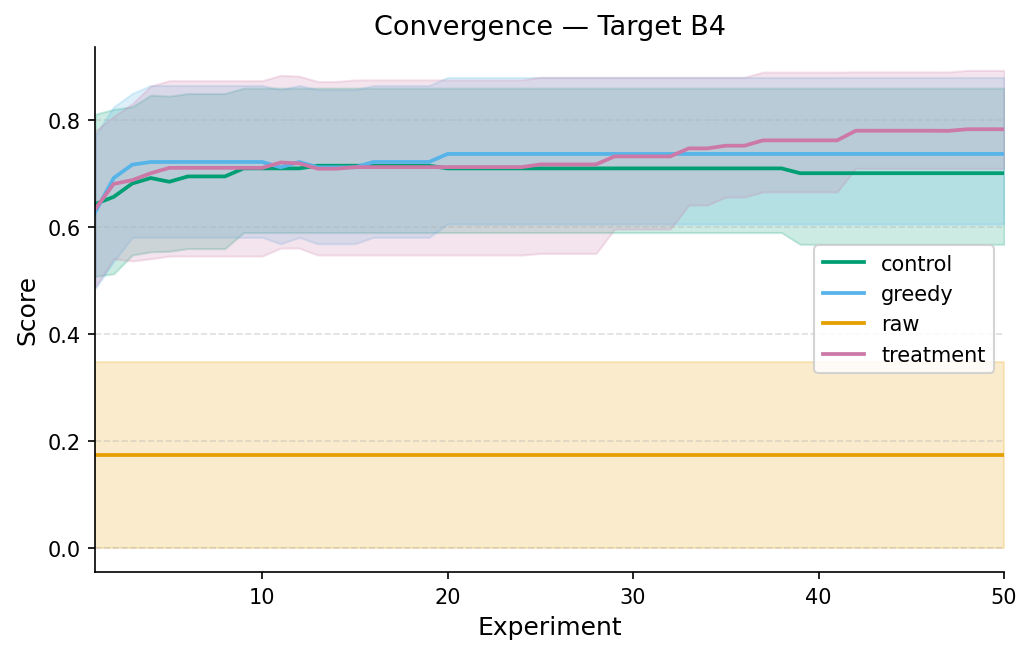
\includegraphics[width=0.195\textwidth]{figures/convergence/convergence_B4.png}\hfill
  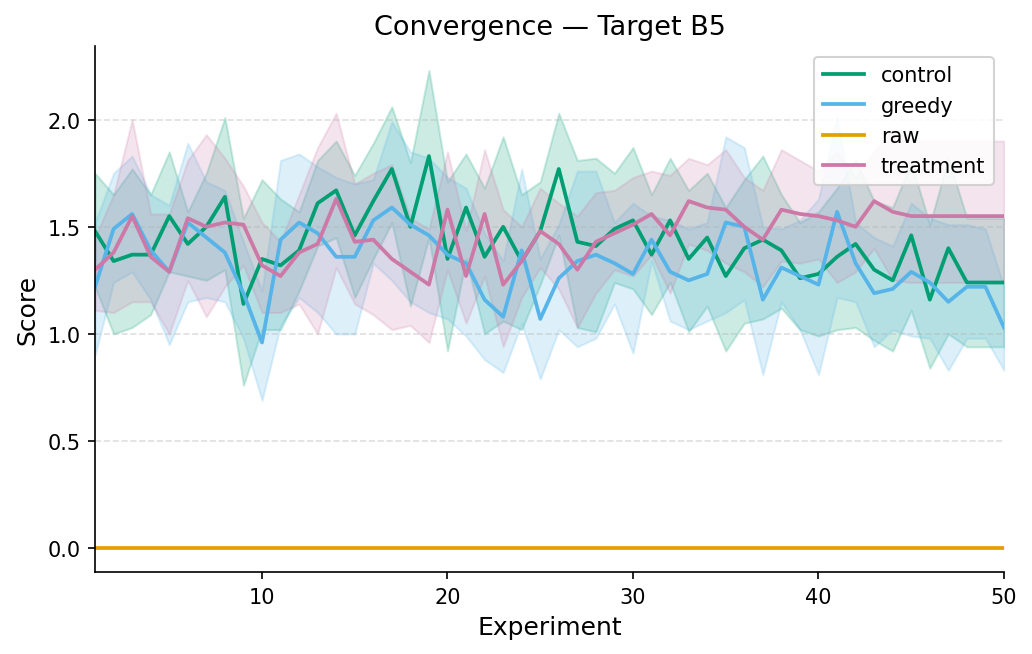
\includegraphics[width=0.195\textwidth]{figures/convergence/convergence_B5.png}
  \Description{Five line plots, one per benchmark target B1 through B5, showing mean final score versus experiment index with one line per configuration (greedy, control, treatment) and shaded standard deviation across the five paired seeds.}
  \caption{Per-experiment convergence trajectories on B1--B5 across the five paired seeds. Each panel plots mean final-score vs.\ experiment index for greedy, control, and treatment; shaded bands show the seed-level standard deviation. Generated by \texttt{benchmarks/analysis/convergence.py} from \texttt{benchmarks/raw\_results\_seeds1-5/}.}
  \label{fig:convergence-strip}
\end{figure*}
The treatment configuration produces a directional improvement over the control configuration on all five targets: $\deltaTCBone\%$ on B1, $\deltaTCBtwo\%$ on B2, $\deltaTCBthreeArith\%$ on B3 (B3 minimizes), $\deltaTCBfour\%$ on B4, and $\deltaTCBfive\%$ on B5.
The treatment configuration also produces a directional improvement over the greedy configuration on all five targets, ranging from $+4.5\%$ on B2 to $+87.8\%$ on B5.
The largest configuration gap is between any optimization configuration and the raw baseline, where the engine reliably moves the artifact away from a starting point that scores zero (B1, B2, B5) or near-zero (B4) on the evaluation rubric.
B3 is noisier: its raw mean is much worse than treatment, while its raw median is zero in the generated summary because several raw executions hit the parser's best-case floor while others are extreme slow outliers.\footnote{The B3 raw-mean (185.68\,ms) and raw-median (0\,ms) divergence reflects this bimodal distribution: roughly half of the seeds produce trivially-fast outputs that the parser clamps at the floor, while the rest are slow outliers that dominate the mean. Treatment mutations bring all five seeds into a compact mid-range distribution, eliminating both modes.}

\begin{table}[t]
  \centering
  \caption{Mean final score per target $\times$ configuration across $n = 5$ paired seeds, with relative change of treatment over control. Direction column indicates whether the metric is maximized ($\uparrow$) or minimized ($\downarrow$).}
  \label{tab:e2e-final-scores}
  \small
  \begin{tabular}{@{}llrrrrr@{}}
    \toprule
    Target & Dir. & raw & greedy & control & treatment & $\Delta_{T/C}$ \\
    \midrule
    B1 & $\uparrow$  & 0.00   & 2.80   & 2.86  & 2.96  & $+3.5\%$  \\
    B2 & $\uparrow$  & 0.00   & 2.68   & 2.54  & 2.80  & $+10.2\%$ \\
    B3 & $\downarrow$ & 185.68 & 103.68 & 72.81 & 40.38 & $-44.5\%$ \\
    B4 & $\uparrow$  & 0.17   & 0.74   & 0.70  & 0.78  & $+11.7\%$ \\
    B5 & $\uparrow$  & 0.00   & 0.82   & 1.30  & 1.54  & $+18.5\%$ \\
    \bottomrule
  \end{tabular}
\end{table}

\subsubsection{Statistical Significance}
\label{sec:end-to-end-significance}

The directional pattern above is consistent across targets, but the framework's own statistical-acceptance discipline is the right standard against which to test it.
\Cref{tab:e2e-stats} reports the Wilcoxon signed-rank $p$-value for each pairwise comparison together with the Holm--Bonferroni-corrected $p$-value across the five targets and Cohen's $d$ with bootstrap 95\% confidence intervals.
The corrected significance threshold is $\alpha = 0.05$.

\begin{table}[t]
  \centering
  \caption{Pairwise comparisons of final score across configurations at $n = 5$ paired seeds per target. $p_{\text{raw}}$ is the Wilcoxon signed-rank $p$-value; $p_{\text{corr}}$ is the Holm--Bonferroni-corrected $p$-value across the five-target family; $d$ is Cohen's $d$ with bootstrap 95\% CI (10{,}000 resamples). Significance is reported at $\alpha = 0.05$ on $p_{\text{corr}}$.}
  \label{tab:e2e-stats}
  \scriptsize
  \begin{tabular}{@{}llrrrl@{}}
    \toprule
    Target & Comparison & $p_{\text{raw}}$ & $p_{\text{corr}}$ & $d$ & 95\% CI \\
    \midrule
    B1 & control vs.\ treatment & 0.625 & 1.000 & 0.18  & $[-1.25, 2.26]$ \\
    B2 & control vs.\ treatment & 0.250 & 1.000 & 0.41  & $[-1.25, 1.96]$ \\
    B3 & control vs.\ treatment & 0.625 & 1.000 & $-0.53$ & $[-2.28, 0.82]$ \\
    B4 & control vs.\ treatment & 0.250 & 1.000 & 0.51  & $[-0.75, 2.25]$ \\
    B5 & control vs.\ treatment & 0.625 & 1.000 & 0.36  & $[-1.25, 1.72]$ \\
    \midrule
    B1 & greedy vs.\ treatment  & 0.250 & 0.750 & 0.26  & $[-1.09, 2.13]$ \\
    B2 & greedy vs.\ treatment  & 0.750 & 1.000 & 0.21  & $[-1.24, 1.76]$ \\
    B3 & greedy vs.\ treatment  & 0.062 & 0.312 & $-1.09$ & $[-3.86, 0.03]$ \\
    B4 & greedy vs.\ treatment  & 0.625 & 1.000 & 0.30  & $[-1.09, 1.74]$ \\
    B5 & greedy vs.\ treatment  & 0.062 & 0.312 & 1.35  & $[\phantom{-}0.46, 3.41]$ \\
    \midrule
    B1 & raw vs.\ treatment     & 0.062 & 0.312 & 6.59  & $[\phantom{-}5.40, 24.96]$ \\
    B2 & raw vs.\ treatment     & 0.062 & 0.312 & 8.00  & $[\phantom{-}6.18, 21.98]$ \\
    B3 & raw vs.\ treatment     & 0.812 & 0.812 & $-0.79$ & $[-2.35, 1.65]$ \\
    B4 & raw vs.\ treatment     & 0.062 & 0.312 & 3.20  & $[\phantom{-}2.64, 13.33]$ \\
    B5 & raw vs.\ treatment     & 0.062 & 0.312 & 3.06  & $[\phantom{-}2.12, \phantom{0}9.30]$ \\
    \bottomrule
  \end{tabular}
\end{table}

\paragraph{What the corrected $p$-values say.}
No comparison reaches significance after Holm--Bonferroni correction at $n = 5$ paired seeds across the five-target family.
The two strongest non-raw signals are the treatment-versus-greedy comparisons on B3 ($d = -1.09$, 95\% CI nearly excludes zero, $p_{\text{corr}} = 0.312$) and on B5 ($d = 1.35$, 95\% CI excludes zero, $p_{\text{corr}} = 0.312$).
Their uncorrected $p$-values are both $0.062$, the smallest the Wilcoxon test can produce at $n = 5$ paired observations: even a perfect 5/5 directional sweep does not clear the corrected threshold under a five-target correction.
The treatment-versus-control effect sizes are small to large across targets ($d \in [-0.53, 0.51]$ on the original sign convention; B3's negative $d$ corresponds to a $44.5\%$ improvement under minimization), and the Wilcoxon test does not reject the null at the corrected threshold.

\paragraph{Why this is the right standard.}
The non-significance of treatment-versus-control after correction is the framework's statistical acceptance discipline applied to itself.
A point-score comparison of the same data would report ``treatment beats control on 5/5 targets'' as a victory; the same comparison run with the engine's own machinery (paired Wilcoxon, multiplicity correction across the five-target family) declines to make that claim at $n = 5$ paired seeds.
The Wilcoxon test's minimum attainable $p$-value at $n = 5$ is $1/2^5 = 0.03125$ for a one-sided test and $0.0625$ for a two-sided test, so even a perfect 5/0 sign sweep within a target sits just above the per-comparison threshold and well above the corrected one.
This is the same conservatism that \cref{sec:gate-false-positives} validated on a synthetic null: the multiplicity correction does not produce false-positive headlines, and at this seed count it requires effect sizes well into Cohen's-large territory or perfect directional consistency in conjunction with a less aggressive correction to reject the null.
The directional pattern across targets and the two strongest B3/B5 greedy-versus-treatment comparisons identify where a higher-powered replication would be most informative.
We discuss this and the implications for interpretation in \cref{sec:threats}.

\subsubsection{Cost Telemetry}
\label{sec:end-to-end-cost}

\Cref{tab:e2e-cost} reports the mean USD cost per seed for the three optimization configurations on each target.
The raw configuration is omitted because it incurs no LLM cost beyond initial-artifact generation.
Treatment cost is within the same order as control cost under the archived model-routing setup: it is higher on B1 and B3, lower on B2, B4, and B5.
Because the archived records were generated under mixed model routing and one draft per experiment (\cref{tab:result-provenance}), these numbers should be interpreted as cost telemetry for this run, not as evidence that specific enhancement mechanisms are cost-neutral.

\begin{table}[t]
  \centering
  \caption{Mean USD cost per seed across configurations, by target (\texttt{total\_cost\_usd} aggregated over the experiment budget, $n = 5$ seeds). These are archived telemetry values under the mixed model-routing setup in \cref{tab:result-provenance}; raw is excluded because its recorded optimization-loop cost is zero.}
  \label{tab:e2e-cost}
  \small
  \begin{tabular}{@{}lrrr@{}}
    \toprule
    Target & greedy (\$) & control (\$) & treatment (\$) \\
    \midrule
    B1 & 2.59 & 2.19 & 2.72 \\
    B2 & 2.64 & 3.12 & 2.86 \\
    B3 & 2.28 & 3.12 & 3.46 \\
    B4 & 1.20 & 1.57 & 1.50 \\
    B5 & 7.56 & 7.53 & 6.71 \\
    \bottomrule
  \end{tabular}
\end{table}

The combined view of \cref{tab:e2e-final-scores,tab:e2e-cost} is that treatment has the strongest directional final scores while remaining within the same cost range as control in this archived run.
The table does not identify which internal feature accounts for cost movement, because the run does not isolate multi-draft, two-phase, dual-agent, or model-routing effects independently.

\subsubsection{Illustrative Trajectory: B4 Code Quality}
\label{sec:end-to-end-illustrative}

To make the abstract numbers concrete, consider one trajectory of the treatment configuration on B4.
The seed artifact is a single-file CRUD endpoint of $\sim 60$ lines: validation absent or stringly-typed, exception handling reduced to a bare \texttt{except} that returns a generic \texttt{500}, timestamps stored as \texttt{str(datetime.now())}, no input bounds, no audit logging.
Under the deterministic composite scorer (correctness via a hidden test suite, plus lint compliance scaled by violation count), this artifact scores $\bar{x}_{\text{raw}} = 0.174$ across the five seeds.
On the first accepted treatment mutation of seed 1, the agent rewrote the file end-to-end: typed pydantic-style request models, explicit email-format and age-range validation with \texttt{422} responses, structured exception handling with distinct status codes for validation versus internal errors, and ISO-formatted timestamps via \texttt{datetime.isoformat}.
The composite score moved from $0.435$ at the seed's pre-experiment baseline to $0.9$ after the mutation, a single-step jump that the framework's statistical-acceptance layer then preserved as the reference baseline for subsequent experiments.
This pattern (a large early jump from the raw artifact, followed by smaller incremental refinements that the multiplicity-corrected acceptance layer admits selectively) is consistent with the per-target descriptive statistics in \cref{tab:e2e-final-scores}.
The full per-experiment trajectories for every seed and configuration are shipped as JSONL in \texttt{benchmarks/raw\_results\_seeds1-5/}.

\subsubsection{Configuration-Step Differences}
\label{sec:end-to-end-ablation}

The four configurations of \cref{tab:e2e-configs} can be read as descriptive steps from less machinery to more machinery, but they do not isolate the independent contribution of each enhancement.
\Cref{tab:e2e-marginal} therefore reports configuration-step differences on the final-score metric, not marginal causal effects.

\begin{table}[t]
  \centering
  \caption{Descriptive configuration-step differences on the final-score metric, per target ($n = 5$ paired seeds). Each cell is the relative change in mean final score between adjacent named configurations. Sign is normalized so that positive numbers represent improvement (B3 minimizes, so its sign is flipped). Cells marked ``--'' are undefined because the raw baseline mean is zero. The rightmost column is the cumulative difference of treatment over raw, where well-defined.}
  \label{tab:e2e-marginal}
  \scriptsize
  \begin{tabular}{@{}lrrrr@{}}
    \toprule
    Target & raw $\to$ greedy & greedy $\to$ control & control $\to$ treatment & raw $\to$ treatment \\
            & (greedy search)  & (+hybrid default) & (+treatment bundle)   & (cumulative)        \\
    \midrule
    B1 & --      & $+2.1\%$  & $+3.5\%$  & -- \\
    B2 & --      & $-5.2\%$  & $+10.2\%$ & -- \\
    B3 & $+44.2\%$ & $+29.8\%$ & $+44.5\%$ & $+78.2\%$ \\
    B4 & $+323\%$  & $-5.0\%$  & $+11.7\%$ & $+350\%$ \\
    B5 & --      & $+58.5\%$ & $+18.5\%$ & -- \\
    \bottomrule
  \end{tabular}
\end{table}

The raw $\to$ greedy column is reported only for targets where the raw mean is non-zero, since percentage change from a zero baseline is undefined.
On the four targets where the greedy $\to$ control transition is well-defined alongside the rest of the chain, control improves over greedy on three of them; the regressions on B2 and B4 are small in absolute terms and within the seed-level standard deviation, consistent with sampling noise at $n = 5$.
The control $\to$ treatment transition is positive on all five targets, ranging from $\deltaTCBone\%$ to $\deltaTCBthree\%$.
This table is useful for locating where the named configurations differ most, but it does not identify which member of the treatment bundle caused the difference.

% ==================================================================
\subsection{Synthesis}
\label{sec:empirical-scope}

The mechanism gates and the end-to-end comparison together establish the strongest claim the data support: the validated subsystems behave as specified in isolation, and the archived treatment configuration improves over greedy hill-climbing and over control on every target in the shipped suite.
The framework's own statistical discipline declines to call this gap significant after multiplicity correction at $n = 5$ paired seeds across the five-target family.
We treat this conservatism as a feature: the same machinery that produced the 86\% false-positive reduction in \cref{sec:gate-false-positives} imposes a stricter standard on systemic claims here, and the strongest B3 and B5 greedy-versus-treatment effects ($d = -1.09$ and $d = 1.35$, $p_{\text{corr}} = 0.312$) identify the comparisons a future higher-powered replication should prioritize.
The threats-to-validity discussion in \cref{sec:threats} elaborates on what the seed count can and cannot resolve, and on the construct-validity considerations specific to LLM-judge evaluation.
